\documentclass[]{article}
\usepackage{lmodern}
\usepackage{amssymb,amsmath}
\usepackage{ifxetex,ifluatex}
\usepackage{fixltx2e} % provides \textsubscript
\ifnum 0\ifxetex 1\fi\ifluatex 1\fi=0 % if pdftex
  \usepackage[T1]{fontenc}
  \usepackage[utf8]{inputenc}
\else % if luatex or xelatex
  \ifxetex
    \usepackage{mathspec}
  \else
    \usepackage{fontspec}
  \fi
  \defaultfontfeatures{Ligatures=TeX,Scale=MatchLowercase}
\fi
% use upquote if available, for straight quotes in verbatim environments
\IfFileExists{upquote.sty}{\usepackage{upquote}}{}
% use microtype if available
\IfFileExists{microtype.sty}{%
\usepackage{microtype}
\UseMicrotypeSet[protrusion]{basicmath} % disable protrusion for tt fonts
}{}
\usepackage[margin=1in]{geometry}
\usepackage{hyperref}
\hypersetup{unicode=true,
            pdftitle={RJDemetra: an R interface to JDemetra+},
            pdfborder={0 0 0},
            breaklinks=true}
\urlstyle{same}  % don't use monospace font for urls
\usepackage{color}
\usepackage{fancyvrb}
\newcommand{\VerbBar}{|}
\newcommand{\VERB}{\Verb[commandchars=\\\{\}]}
\DefineVerbatimEnvironment{Highlighting}{Verbatim}{commandchars=\\\{\}}
% Add ',fontsize=\small' for more characters per line
\usepackage{framed}
\definecolor{shadecolor}{RGB}{248,248,248}
\newenvironment{Shaded}{\begin{snugshade}}{\end{snugshade}}
\newcommand{\KeywordTok}[1]{\textcolor[rgb]{0.13,0.29,0.53}{\textbf{#1}}}
\newcommand{\DataTypeTok}[1]{\textcolor[rgb]{0.13,0.29,0.53}{#1}}
\newcommand{\DecValTok}[1]{\textcolor[rgb]{0.00,0.00,0.81}{#1}}
\newcommand{\BaseNTok}[1]{\textcolor[rgb]{0.00,0.00,0.81}{#1}}
\newcommand{\FloatTok}[1]{\textcolor[rgb]{0.00,0.00,0.81}{#1}}
\newcommand{\ConstantTok}[1]{\textcolor[rgb]{0.00,0.00,0.00}{#1}}
\newcommand{\CharTok}[1]{\textcolor[rgb]{0.31,0.60,0.02}{#1}}
\newcommand{\SpecialCharTok}[1]{\textcolor[rgb]{0.00,0.00,0.00}{#1}}
\newcommand{\StringTok}[1]{\textcolor[rgb]{0.31,0.60,0.02}{#1}}
\newcommand{\VerbatimStringTok}[1]{\textcolor[rgb]{0.31,0.60,0.02}{#1}}
\newcommand{\SpecialStringTok}[1]{\textcolor[rgb]{0.31,0.60,0.02}{#1}}
\newcommand{\ImportTok}[1]{#1}
\newcommand{\CommentTok}[1]{\textcolor[rgb]{0.56,0.35,0.01}{\textit{#1}}}
\newcommand{\DocumentationTok}[1]{\textcolor[rgb]{0.56,0.35,0.01}{\textbf{\textit{#1}}}}
\newcommand{\AnnotationTok}[1]{\textcolor[rgb]{0.56,0.35,0.01}{\textbf{\textit{#1}}}}
\newcommand{\CommentVarTok}[1]{\textcolor[rgb]{0.56,0.35,0.01}{\textbf{\textit{#1}}}}
\newcommand{\OtherTok}[1]{\textcolor[rgb]{0.56,0.35,0.01}{#1}}
\newcommand{\FunctionTok}[1]{\textcolor[rgb]{0.00,0.00,0.00}{#1}}
\newcommand{\VariableTok}[1]{\textcolor[rgb]{0.00,0.00,0.00}{#1}}
\newcommand{\ControlFlowTok}[1]{\textcolor[rgb]{0.13,0.29,0.53}{\textbf{#1}}}
\newcommand{\OperatorTok}[1]{\textcolor[rgb]{0.81,0.36,0.00}{\textbf{#1}}}
\newcommand{\BuiltInTok}[1]{#1}
\newcommand{\ExtensionTok}[1]{#1}
\newcommand{\PreprocessorTok}[1]{\textcolor[rgb]{0.56,0.35,0.01}{\textit{#1}}}
\newcommand{\AttributeTok}[1]{\textcolor[rgb]{0.77,0.63,0.00}{#1}}
\newcommand{\RegionMarkerTok}[1]{#1}
\newcommand{\InformationTok}[1]{\textcolor[rgb]{0.56,0.35,0.01}{\textbf{\textit{#1}}}}
\newcommand{\WarningTok}[1]{\textcolor[rgb]{0.56,0.35,0.01}{\textbf{\textit{#1}}}}
\newcommand{\AlertTok}[1]{\textcolor[rgb]{0.94,0.16,0.16}{#1}}
\newcommand{\ErrorTok}[1]{\textcolor[rgb]{0.64,0.00,0.00}{\textbf{#1}}}
\newcommand{\NormalTok}[1]{#1}
\usepackage{graphicx,grffile}
\makeatletter
\def\maxwidth{\ifdim\Gin@nat@width>\linewidth\linewidth\else\Gin@nat@width\fi}
\def\maxheight{\ifdim\Gin@nat@height>\textheight\textheight\else\Gin@nat@height\fi}
\makeatother
% Scale images if necessary, so that they will not overflow the page
% margins by default, and it is still possible to overwrite the defaults
% using explicit options in \includegraphics[width, height, ...]{}
\setkeys{Gin}{width=\maxwidth,height=\maxheight,keepaspectratio}
\IfFileExists{parskip.sty}{%
\usepackage{parskip}
}{% else
\setlength{\parindent}{0pt}
\setlength{\parskip}{6pt plus 2pt minus 1pt}
}
\setlength{\emergencystretch}{3em}  % prevent overfull lines
\providecommand{\tightlist}{%
  \setlength{\itemsep}{0pt}\setlength{\parskip}{0pt}}
\setcounter{secnumdepth}{0}
% Redefines (sub)paragraphs to behave more like sections
\ifx\paragraph\undefined\else
\let\oldparagraph\paragraph
\renewcommand{\paragraph}[1]{\oldparagraph{#1}\mbox{}}
\fi
\ifx\subparagraph\undefined\else
\let\oldsubparagraph\subparagraph
\renewcommand{\subparagraph}[1]{\oldsubparagraph{#1}\mbox{}}
\fi

%%% Use protect on footnotes to avoid problems with footnotes in titles
\let\rmarkdownfootnote\footnote%
\def\footnote{\protect\rmarkdownfootnote}

%%% Change title format to be more compact
\usepackage{titling}

% Create subtitle command for use in maketitle
\newcommand{\subtitle}[1]{
  \posttitle{
    \begin{center}\large#1\end{center}
    }
}

\setlength{\droptitle}{-2em}

  \title{RJDemetra: an R interface to JDemetra+}
    \pretitle{\vspace{\droptitle}\centering\huge}
  \posttitle{\par}
    \author{}
    \preauthor{}\postauthor{}
    \date{}
    \predate{}\postdate{}
  
\usepackage{float}

\begin{document}
\maketitle

\section{Introduction}\label{introduction}

RJDemetra is a R interface to
\href{https://github.com/jdemetra/jdemetra-app}{JDemetra+}, the seasonal
adjustment software
\href{https://ec.europa.eu/eurostat/cros/system/files/Jdemetra_\%20release.pdf}{officially
recommended} to the members of the ESS and the European System of
Central Banks.

JDemetra+ is a developed by the National Bank of Belgium (NBB) in
cooperation with the Deutsche Bundesbank and Eurostat in accordance with
the Guidelines of the European Statistical System (ESS). It implements
the two leading seasonal adjustment methods
\href{http://www.bde.es/bde/en/secciones/servicios/Profesionales/Programas_estadi/Programas_estad_d9fa7f3710fd821.html}{TRAMO/SEATS+}
and
\href{https://www.census.gov/srd/www/x13as/}{X-12ARIMA/X-13ARIMA-SEATS}.

R is a programming language and free software environment for
statistical computing and free software widely use by statisticians.

RJDemetra is a R package that offers full access to all options and
outputs of JDemetra+. It also offers many possibilities to the users of
JDemetra+ to implements new tools for the production of seasonally
adjusted series thanks to all the libraries already available in R. It's
available in github: \url{https://github.com/nbbrd/RJDemetra}.

\section{Methods}\label{methods}

RJDemetra relies on the Java libraries use in JDemetra+: the algorithms
are not implemented inside the package. The link between R and Java
libraries is done with the
\href{https://CRAN.R-project.org/package=rJava}{rJava} package, which is
a low-level R to Java interface. The consequence is that the results of
the seasonal adjustment done in R are certified by the use of JDemetra+
and the system requirements needed to install the package are the same
needed to use JDemetra+ (Java SE 8 or later).

The goal of the RJDemetra package is to offer a ``pure R'' package to
the users, more familiar to this language rather that Java. It allows
them to integrate easily the seasonal adjustment process it their
production and offers the possibility to implements new tools that are
difficult to integrate into the graphical interface of JDemetra+, for
example:

\begin{itemize}
\tightlist
\item
  comparison of the direct and indirect aggregates adjustment;\\
\item
  automatic generation of dashboards to summarise information for people
  responsible of the ongoing production but not of the maintenance of
  the seasonally adjusted models (and so non-JDemetra+ users);\\
\item
  more easily implement quality report procedures.
\end{itemize}

\section{Results}\label{results}

In the current version of the RJDemetra package, users can:

\begin{itemize}
\tightlist
\item
  seasonally adjust their time series with the TRAMO-SEATS and
  X-13-ARIMA methods;\\
\item
  use the regARIMA preadjustment method implemented in TRAMO-SEATS and
  X-13-ARIMA methods;\\
\item
  manipulate JDemetra+ workspace to easily switch from R models to the
  JDemetra+ graphical interface. The current functionalities are:

  \begin{itemize}
  \tightlist
  \item
    importing JDemetra+ workspace in R to get input raw series or the
    seasonally adjust model as defined in RJDemetra;
  \item
    exporting R models created via RJDemetra to a readable JDemetra+
    workspace.
  \end{itemize}
\end{itemize}

All the seasonally adjust object created by RJDemetra are S3 classes
with basic methods implements: \texttt{print()}, \texttt{plot()} and
\texttt{summary()} (for regARIMA models).

Let's see an example with the French industrial production index in
manufacturing
(\url{https://www.insee.fr/en/statistiques/serie/010537903}). The time
series can be seasonally adjusted with the X-13-ARIMA method by the
function \texttt{x13\_def()}: main results are presented in figure
\ref{fig:sa_ipi} created by the \texttt{plot()} function.

\begin{Shaded}
\begin{Highlighting}[]
\KeywordTok{library}\NormalTok{(RJDemetra)}
\NormalTok{x13_ipi <-}\StringTok{ }\KeywordTok{x13_def}\NormalTok{(ipi_french, }\DataTypeTok{spec =} \StringTok{"RSA3"}\NormalTok{)}
\KeywordTok{print}\NormalTok{(x13_ipi,}\DataTypeTok{enable_print_style =} \OtherTok{FALSE}\NormalTok{)}
\end{Highlighting}
\end{Shaded}

\begin{verbatim}
## 
## 
## RegARIMA
## y = regression model + arima (3, 0, 0, 0, 1, 1)
## Log-transformation: yes
## Coefficients:
##           Estimate Std. Error
## Phi(1)     0.06496      0.060
## Phi(2)    -0.22318      0.058
## Phi(3)    -0.53899      0.059
## BTheta(1) -0.87452      0.044
## 
##               Estimate Std. Error
## Mean          0.003291      0.002
## LS (11-2008) -0.127329      0.016
## 
## 
## Residual standard error: 0.02923 on 212 degrees of freedom
## Log likelihood = 439.1, aic =  1107 aicc =  1107, bic(corrected for length) = -6.914
## 
## 
## 
## Decomposition
## Monitoring and Quality Assessment Statistics: 
##       M stats
## M(1)    0.407
## M(2)    0.377
## M(3)    3.000
## M(4)    0.062
## M(5)    3.000
## M(6)    0.526
## M(7)    0.142
## M(8)    0.330
## M(9)    0.065
## M(10)   0.311
## Q       0.845
## Q-M2    0.903
## 
## Final filters: 
## Seasonal filter:  3x5
## Trend filter:  23-Henderson
## 
## 
## Final
## Last observed values
##               y       sa        t         s         i
## Sep 2017 108.54 102.2883 103.7189 1.0611187 0.9862062
## Oct 2017 113.60 104.8975 103.7928 1.0829621 1.0106431
## Nov 2017 110.70 107.2133 103.8364 1.0325213 1.0325214
## Dec 2017  97.97 101.4844 103.8632 0.9653705 0.9770966
## Jan 2018 102.92 106.2211 103.8905 0.9689223 1.0224332
## Feb 2018  99.45 103.1341 103.9304 0.9642786 0.9923378
## Mar 2018 112.96 103.6153 103.9858 1.0901868 0.9964372
## Apr 2018 103.38 102.3360 104.0587 1.0102017 0.9834449
## May 2018  99.27 102.7787 104.1677 0.9658616 0.9866661
## Jun 2018 112.60 103.7506 104.3134 1.0852952 0.9946043
## Jul 2018 106.76 106.7344 104.4946 1.0002399 1.0214348
## Aug 2018  82.14 106.0951 104.6781 0.7742111 1.0135370
## 
## Forecasts:
##                y_f     sa_f      t_f       s_f       i_f
## Sep 2018 110.17751 104.1644 104.8277 1.0577272 0.9936725
## Oct 2018 113.97238 105.2478 104.9164 1.0828954 1.0031594
## Nov 2018 108.36831 104.5309 104.9059 1.0367111 0.9964247
## Dec 2018 100.66007 104.6131 104.8079 0.9622127 0.9981419
## Jan 2019 101.78559 104.7078 104.6226 0.9720916 1.0008141
## Feb 2019 101.18138 105.0994 104.3965 0.9627208 1.0067329
## Mar 2019 112.46321 103.0487 104.1593 1.0913602 0.9893369
## Apr 2019 105.06030 104.2347 103.9424 1.0079205 1.0028124
## May 2019 100.34816 103.6569 103.7215 0.9680800 0.9993770
## Jun 2019 112.79333 104.1444 103.4615 1.0830472 1.0066012
## Jul 2019 104.40231 104.4259 103.2479 0.9997741 1.0114093
## Aug 2019  78.32815 100.9817 103.0722 0.7756672 0.9797177
## 
## 
## Diagnostics
##  Relative contribution of the components to the stationary portion of the variance in the original series, after the removal of the long term trend 
##  Trend computed by Hodrick-Prescott filter (cycle length = 8.0 years)
##            Component
##  Cycle         2.148
##  Seasonal     66.591
##  Irregular     4.205
##  TD & Hol.     0.000
##  Others       27.124
##  Total       100.068
## 
##  Residual seasonality tests 
##                                       P.value
##  qs test on sa                          0.017
##  qs test on i                              NA
##  f-test on sa (seasonal dummies)        0.930
##  f-test on i (seasonal dummies)            NA
##  Residual seasonality (entire series)   0.941
##  Residual seasonality (last 3 years)    0.912
##  f-test on sa (td)                      0.000
##  f-test on i (td)                          NA
## 
##  Combined test in the entire series 
##  Non parametric tests for stable seasonality
##                                                           P.value
##    Kruskall-Wallis test                                      0.000
##    Test for the presence of seasonality assuming stability   0.000
##    Evolutive seasonality test                                0.955
##  
##  Identifiable seasonality present
## 
##  Combined test in the last 3 years 
##  Non parametric tests for stable seasonality
##                                                           P.value
##    Kruskall-Wallis test                                      0.002
##    Test for the presence of seasonality assuming stability   0.000
##    Evolutive seasonality test                                0.212
##  
##  Identifiable seasonality probably present
## 
## 
## Additional output variables
\end{verbatim}

\begin{Shaded}
\begin{Highlighting}[]
\KeywordTok{plot}\NormalTok{(x13_ipi, }\DataTypeTok{type_chart =} \StringTok{"sa-trend"}\NormalTok{)}
\end{Highlighting}
\end{Shaded}

\begin{figure}
\centering
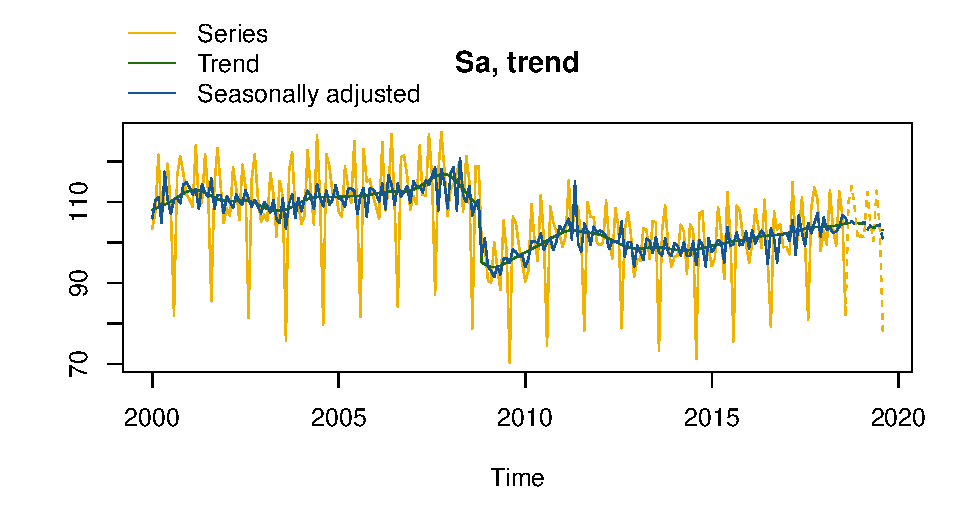
\includegraphics{NTTS_files/figure-latex/unnamed-chunk-2-1.pdf}
\caption{\label{fig:sa_ipi}The result of the seasonal adjustment process
for the french IPI in manufacturing}
\end{figure}

More complex figures are also implemented to have more details on the
decomposition of the model, like S-I-ratio (figures
\ref{fig:sa_si_ratio}).

\begin{Shaded}
\begin{Highlighting}[]
\KeywordTok{plot}\NormalTok{(x13_ipi}\OperatorTok{$}\NormalTok{decomposition, }\DataTypeTok{ask =} \OtherTok{FALSE}\NormalTok{)}
\end{Highlighting}
\end{Shaded}

\begin{figure}
\centering
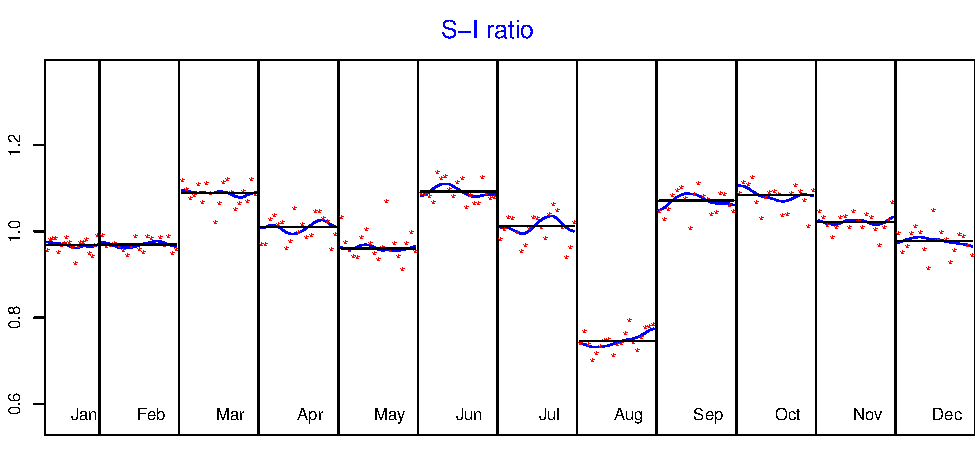
\includegraphics{NTTS_files/figure-latex/unnamed-chunk-3-1.pdf}
\caption{\label{fig:sa_si_ratio}S-I ratio}
\end{figure}

Other R libraries can also be used on the result of the seasonal
adjustment model, not available in JDemetra+. So, for example, the
Diebold-Mariano test (implemented in the
\href{ttps://CRAN.R-project.org/package=forecast}{forecast} package) can
be used to compare the forecast accuracy of two regARIMA models,as the
Shapiro-Wilk test of normality on the residuals of a regARIMA model:

\begin{Shaded}
\begin{Highlighting}[]
\KeywordTok{shapiro.test}\NormalTok{(x13_ipi}\OperatorTok{$}\NormalTok{regarima}\OperatorTok{$}\NormalTok{residuals)}
\end{Highlighting}
\end{Shaded}

\begin{verbatim}
## 
##  Shapiro-Wilk normality test
## 
## data:  x13_ipi$regarima$residuals
## W = 0.99401, p-value = 0.5564
\end{verbatim}

\section{Conclusions}\label{conclusions}

Implemen


\end{document}
